\chapter{Introduction}
\label{chap:introduction}

Altough high temperature superconductivity has been known for almost three decades \cite{Bednorz1986}, a satisfactory explanation of this phenomenom still remains as one of the major unsolved problems in theoretical condensed matter physics. 
It is known that, similarly to BCS theory \cite{Bardeen1957}, high-temperature superconductivity is caused by attraction between electrons \cite{?}. 
However it remains unclear how this attraction arises, when it is sizable and when it is not, and what factors are detrimental to superconductivity.

The high-T$_c$ cuprate superconductors have complex phase diagrams with many competing ground states and quantum phase transitions between them \cite{Chakravarty2011}.
Parent compounds of copper based superconductors start out as insulators and become superconductors when doped with additional charge carriers.
Depending on the compound, superconducting charge carriers can be either electrons or holes.
We show a simplified phase diagram for several cuprate superconductors in Figure \ref{fig:CuPhaseDiag} which highlights some of common characteristics between them.
For low charge carriers concentration the parent compounds form ordered crystalline structures and exhibit antiferromagnetism below a certain temperature $T_N$ \cite{?}.
This antiferromagnetic phase is suppresed by charge doping giving rise to superconductivity.
Antiferromagnetism and superconductivity seem to be excluyent \cite{?}, however they appear in close proximity in the phase diagram.
After the antiferromagnetism is suppressed, the superconducting transition temperature (T$_c$) rises with doping until it reaches a maximum value for some optimal doping level finally decreasing to zero for greater dopings.

\begin{figure}[ht]
  \centering
  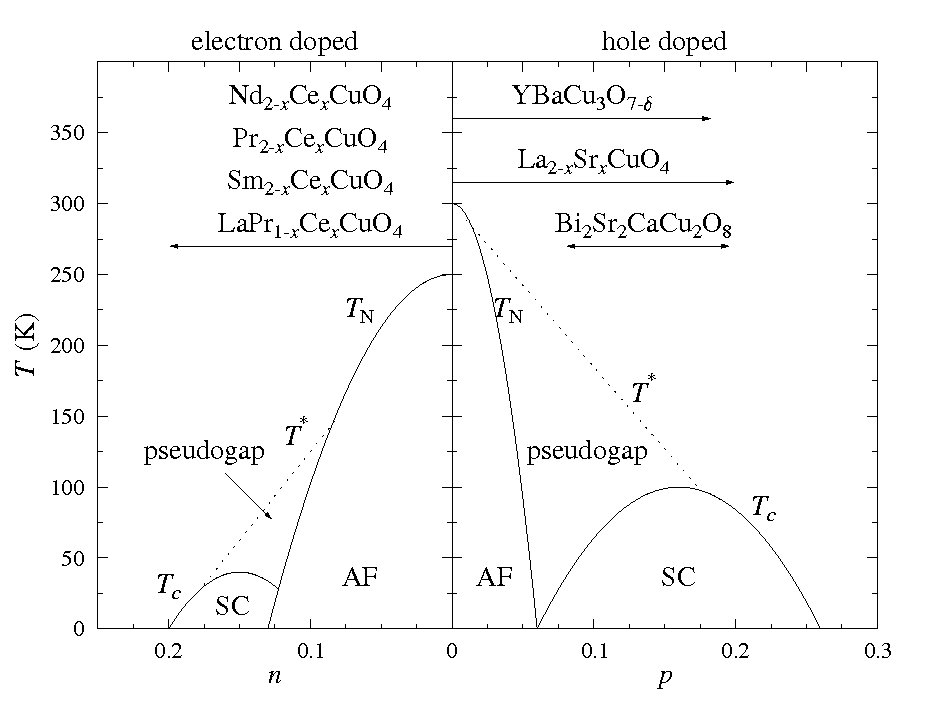
\includegraphics[width=0.8\textwidth]{images/CuPhaseDiag.png}
  \caption[Simplified version of the cuprate superconductor phase diagram]
  {Simplified version of the cuprate superconductor phase diagram \protect\cite{CuPhaseDiag}.}
  \label{fig:CuPhaseDiag}
\end{figure}

One defining property of a superconductor, within the band energy approximation, is the presence of an energy gap, but early experiments could not find its characteristic signatures in cuprate superconductors.
Instead of abruptly finding a zero density of states below a certain energy at the superconducting transition temperature there was only a partial depression of excitations appearing at a much higher temperature T*.
This region of phase space has been identified as the \textit{pseudogap phase} and there is evidence for its presence in all cuprate superconductor families \cite{Timusk1999,Muller2007}.
This phase seems to precede superconductivity for a large part of the phase diagram but its relationship to superconductivity still remains unclear \cite{?}.

In addition to the partial gap, the pseudogap phase presents many interesting characteristics. 
One of them is the observation of lattice inhomogeneities, for example in La$_{1.85}$Sr$_{0.15}$CuO$_{4}$ and La$_{2}$CuO$_{4.1}$, the dopant atoms, necessary for superconductivity, do not reside at the crystal symmetric sites making these compounds structurally inhomogeneous \cite{Poccia2011}.
In YBa$_2$Cu$_3$O$_{7-\delta}$ (YBCO) the dopant atoms reside in crystal symmetric positions but the departure from stoichiometry produces compositional disorder \cite{Chen1988,Andersen1990} making YBCO also an inhomogeneous system.
Even though the dopant atoms are at fixed positions, these structural inhomogeneities have a dynamical character \cite{Mihailovic2005,Bianconi1996}.
Such a dynamical inhomogeneity is present even in some compounds with perfect crystallographic symmetry like HoBa$_{2}$Cu$_{4}$O$_{8}$ \cite{RubioTemprano2000}.
Although from the structural inhomogeneity does not necessarily follow an inhomogeneous electronic ground state, for some regions of the phase diagram, depending on the dopant concentation, such state is realized.
In these systems the crystalline translational symmetry is broken. 

In addition to the breaking of the crystalline translational symmetry the pseudogap phase exhibits other broken symmetries. 
Time-reversal symmetry breaking was found using angular resolved photoemission spectroscopy with circularly polarized photons in Bi$_{2}$Sr$_{2}$CaCu$_{2}$O$_{8+\delta}$ \cite{Kaminski2002}. 
It was also found, by x-ray absorption spectroscopy, that the crystalline rotational symmetry is broken locally in La$_{1.85}$Sr$_{0.15}$CuO$_{4}$ with alternating regions of tetragonal and orthorhombic symmetry \cite{Bianconi1996}.  
This \textit{inherent inhomogeneity} in HTSC observed by many techniques (see paragraph 2 of \cite{Bussmann-Holder2005}).

The clues provided by these broken symmetries should yield an understanding of the ground state in this pseudogap phase, its elementary excitations and the appearance of superconductivity at temperatures below the onset of the pseudogap. 


\cite{Kresin2009}: ``Electron-lattice interaction and its impact in high-T$_c$ superconductivity'' (polaronic nature of the carriers)

In the remainder of this introduction we briefly review the manifestation of the lattice inhomogeneity and the charge-lattice coupling in several experimental techniques.

This charge-lattice dynamic is inaccessible within the Born-Oppenheimer approximation, thus an exact treatment is necessary.
We focus on a small but important subsytem and study a model hamiltonian for it that explains some of the experimental evidence

The clues provided by these broken symmetries should yield an understanding of the ground state in this pseudogap phase, its elementary excitations and the appearance of superconductivity at temperatures below the onset of the pseudogap. 

The remainder of this introductory chapter is devoted to reviewing some of the experimental results pointing to the importance of considering the lattice and electronic inhomogeneities in the description of superconductivity. 
We start, in section \ref{sec:dynamicDistortions} with an overview of the dynamic local lattice distortions in cuprates incluiding the important feature of stripes. 
Afterwards, in section \ref{sec:electronic_inhomogeneity}, we turn our attention to electronic inhomogeneities. 
In sections \ref{sec:phonon_spectra} and \ref{sec:specific_heat} we present some experimental anomalies in the phonon spectra and specific heat respectively and speculate about their possible origin in the mentioned inhomogeneities. 
Next we duscuss some of the controversial experimental results in isotopic effects and ultrafast spectroscopy in sections \ref{sec:isotopic_effects} and \ref{sec:ultrafast_spect} respectively.

In the last part of this introduction we limit the scope of this thesis and present our motivation and approach at describing these dynamic effects (sec. \ref{sec:scope}) and provide an outline of the next chapters.

\section{Purely electronic theories}
\label{sec:electronicTheories}

In contrast to the BCS theory \cite{Bardeen1957}, the pairing mechanism in the \textit{unconventional superconductors} (cuprates, iron-based and heavy fermion \cite{Pfleiderer2009}) is unknown.
Two leading theories: resonating-valence-bond \cite{?} and spin fluctuation \cite{Scalapino2012} rely heavily on magnetic interactions while mostly ignoring the lattice effects.

Soon after their discovery Anderson proposed \cite{Anderson1987} that the parent compounds are in a \textit{quantum spin liquid} phase that do not break any symmetries. 

In this theory, also called the \textit{resonating valence bond} (RVB), he argues that
\begin{quote}
  The preexisting magnetic singlet pairs of the insulating state become charged superconducting pairs when the insulator is doped sufficiently strongly. 
The mechanism for superconductivity is hence predominantly electronic and magnetic, although weak phonon interactions may favor the state.
\end{quote} 

\cite{Chakravarty2008}: Breaking of RVB


\section{Dynamic local lattice distortions}
\label{sec:dynamicDistortions}

From https://research-engine.appspot.com/37001/writings/6264610306916352

\begin{quote}
Early determinations of the crystal structure of cuprates by diffraction methods did not show significant distortions associated with either in-plane oxygen atoms or apical oxygen atoms \cite{Capponi1987,Schafer1988}. 
Moreover, the determination of  average bond lengths in diffraction has a precision of $\sim 0.001$\AA \cite{Miceli1988}, significantly higher than the precision in bond length determination that local probes, like extended x-ray absorption fine structure spectroscopy (EXAFS) \cite{Rehr2000}. 
For this reason, early reports of local lattice distortions related to the oxygen atoms  were controversial (see for example \cite{battlog1992lattice,Kwei1990}).

One of the first observations of a local lattice distortion in cuprates was the report of a two-site distribution for the Cu(1)-apical oxygen in YBa$_{2}$Cu$_{3}$O$_{7}$  appearing at temperatures above the superconducting transition temperature, T$_{c}$, using Cu K-edge EXAFS \cite{MustredeLeon1990,Conradson1990}.
This distribution showed two sites separated by $\sim 0.10-0.13$ \AA \cite{Conradson1990,MustredeLeon1992a} that changed into a single site distribution in the vicinity of the superconducting transition temperature. 
These measurements were carried out using polarized x-rays on magnetically oriented powders, an improvement in the technique which allowed to isolate the Cu(1)-axial oxygen [O(4)] (see Fig. 1) signal with an increased sensitivity not achievable for the Cu-O EXAFS signal in other cuprates (see below). 
This result was received with skepticism, based on earlier diffraction results \cite{battlog1992lattice,Kwei1990,Sharma1991} and optical spectroscopy \cite{Thomsen1993}. 
However, it was later confirmed by EXAFS measurements in other oriented samples \cite{Stern1993} and single crystals \cite{Booth1996}, and also found in YBa$_{2}$Cu$_{3}$O$_{6.7}$, YBa$_{2}$Cu$_{3}$O$_{6.5}$ and Co doped YBa$_{2}$Cu$_{3}$O$_{7}$ \cite{MustredeLeon1991}. 
The explanation of the discrepancies between these results with diffraction and optical spectroscopical results lead to the interpretation of  this Cu(1)-O(4) distribution as a dynamical distortion of polaronic origin \cite{MustredeLeon1992}, as discussed in the next section.

Similar two site distributions obtained from EXAFS spectra were found for the Cu(2)-O(4) distribution in Bi$_{2}$Sr$_{2}$CaCu$_{2}$O$_{8}$ \cite{bianconni1992lattice} and in TlBa$_{2}$Ca$_{3}$Cu$_{4}$O$_{11}$ \cite{Allen1991} starting at temperatures above T$_{c}$. 
We note that in these compounds (and other cuprates) the average Cu(2)-O(4) bond length lies between 2.49 and $2.73$ \AA, which is much longer than the Cu(1)-O(4) bond length in YBa$_{2}$Cu$_{3}$O$_{7}$ $(\sim 1.87$ \AA). 
This fact makes more difficult the identification of details of the O(4) distribution due to the stronger mixing of the Cu(2)-O(4) EXAFS signal with those of other atoms and the increased zero point motion of the O(4) atom due to weaker Cu(2)-O(4) bond compared with the Cu(1)-O(4) bond.
For this reason in most EXAFS studies addressing the O(4) motion a gaussian single site broadened distribution has been used, reporting only changes in the width of the distribution as a function of temperature \cite{Booth1995,Oyanagi2007,Zhang2009}.

In plane  Cu(2)-O local lattice distortions were identified in La$_{1.85}$Sr$_{0.15}$CuO$_{4}$ appearing below 100 K \cite{Bianconi1996,Oyanagi2007},  in TIBa$_{2}$CuO$_{6}$ below 120 K \cite{Conradson1997} and in La$_{2}$CuO$_{4.1}$ below 150 K \cite{Lanzara1997,MustredeLeon:xj5003}. 
In this case the observation of such distortions in YBa$_{2}$Cu$_{3}$O$_{7}$ and related compounds becomes more difficult due the similarity  in Cu-O bond lengths in the Cu planes and Cu chains, whose contributions are mixed in the EXAFS signal \cite{Conradson1997,MustredeLeon1992a}.

Until now only in La$_{1.85}$Sr$_{0.15}$CuO$_{4}$ has been possible to identify local lattice distortions involving both in plane oxygen and apical oxygen atoms  \cite{Bianconi1996}. 
We also stress that from all these EXAFS experiments it is only possible to probe with enough detail the nearest neighbor environment around the Cu atoms, thus the spatial extension of the distortions cannot be determined solely from these measurements. 
Additional structural information \cite{Bianconi1996a} is needed to formulate models about the extension of the distortions as discussed in Ref. \cite{Bianconi1996}.

Pair distribution function (PDF) analysis of diffraction, x-ray and neutron inelastic scattering can additionally provide information about the intermediate range (up to $10-15$ \AA)  atomic structure, complementary to the information obtained from EXAFS \cite{Egami2003}. 
PDF results in La$_{1-x}$Sr$_{x}$CuO$_{4}$ \cite{Bozin1999,Bozin2000} indicate that the atomic structure in this material is a combination of nanoscale regions with different local Cu-O environments, in agreement with the model proposed in Ref. \cite{Bianconi1996}. 
A homogeneous structure only appears when dopant concentrations are above $x = 0.25$. 
In this region the electronic behavior can be described in terms of free fermion quasiparticles.

To conclude this survey of local lattice distortion is important to note that the time scale of the EXAFS is such that dynamical distortions can be detected, which depending on the size of the distortion cannot be detected using elastic techniques like neutron diffraction (see section of Results). 
This can explain some of the differences between diffraction and EXAFS results. 
Indeed it has been shown that the two-site O(4) distribution in in Tl$_{2}$Ba$_{2}$CaCu$_{2}$O$_{8}$ could be only detected in a pair distribution function obtained from neutron inelastic scattering but not with that obtained from neutron diffraction \cite{Egami1991}. 
Consequently, it is important to take into account both the spatial resolution and time resolution of the techniques used to study the actual atomic structure of these materials \cite{Mihailovic2005}. 
In the next section we present a microscopic local model that can generate  dynamical local lattice distortions as those observed in these materials, and explain the isotopic effects observed in the pseudogap phase.
\end{quote}

\begin{figure}[ht]
  \centering
  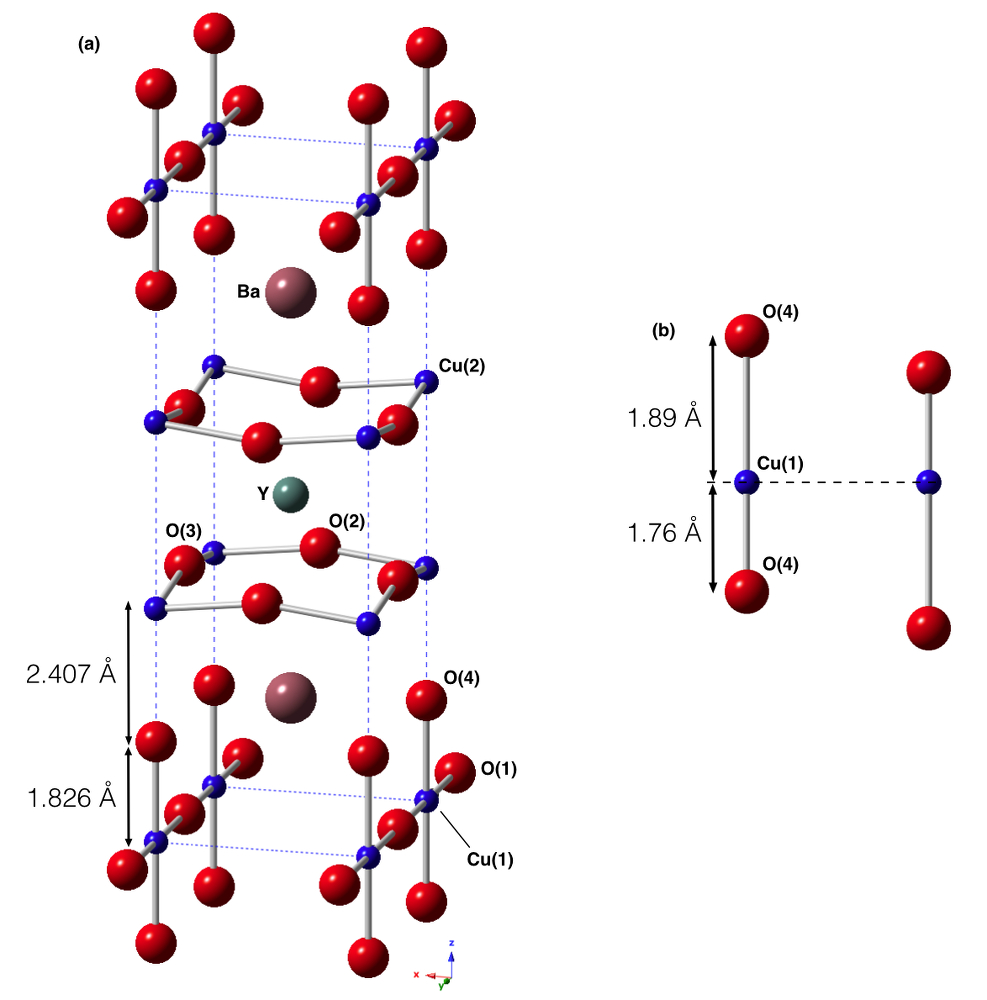
\includegraphics[width=0.8\textwidth]{images/YBCO_O-Cu-O.jpg}
  \caption[Crystal structure of YBa$_{2}$Cu$_{3}$O$_{7}$ and the two possible O(4)-Cu(1)-O(4) configurations.]
  {\textbf{(a)} Crystal structure of YBa$_{2}$Cu$_{3}$O$_{7}$. The dashed line denotes de unit cell. \textbf{(b)} The two possible configurations in the O(4)-Cu(1)-O(4) cluster due to the split O-Cu bond distances (not to scale).}
\label{fig:YBCO_structure}
\end{figure}

From \cite{Bahrs2004}

\begin{quote}
Samples quenched from high to about room temperature show spontaneous reordering of oxygen atoms in the chain sites on a time scale between hours and days. 
The structural development has been monitored with x-ray and neutron scattering, both verifying a shortening of the crystallographic axes and the formation of superstructure patterns with full and empty chains for values of oxygen deficiency around $\delta \sim  0.5$. 
[...] the critical temperature of the samples was observed to increase, pointing to the close connection between chain length and carrier concentration in the superconducting planes. 
Calculations of the Cu1 valence in different oxygen surroundings explain the charge transfer involved. 
This correlation between structure and electrical properties has also been shown by application of pressure, after which the critical temperature also remains enhanced as long as the sample is kept cool, but relaxes when it is warmed up to room temperature. 
Other metastable effects are induced by illumination, such as persistent photoconductivity, where after exposure to visible light conductivity and, in superconducting samples, critical temperature show a metastable increase.
\end{quote}

Stripes review: \cite{Kivelson2003}

\section{Electronic inhomogeneity}
\label{sec:electronic_inhomogeneity}

STM observations of electronic inhomogeneity in Bi$_2$Sr$_2$CaCu$_2$O$_{8+\delta}$ http://www.nature.com/nature/journal/v413/n6853/full/413282a0.html

Charge density variations through NMR in YBa$_2$Cu$_3$O$_{7-\delta}$
http://link.springer.com/article/10.1023%2FA%3A1023882516857

See introduction of this article: \cite{Ivanov1995}

ARPES review: \cite{Damascelli2003}

\section{Phonon spectra}
\label{sec:phonon_spectra}

Forbidden ir modes only present below T* \cite{?}

``Phonon contributions to the specific heat as a function of Co content correlate closely with observed anomalies in calorimetric measurements, indicating that phonons contribute intrinsically to the transition mechanism, e.g. via Bose condensation of structural bipolarons.'' \cite{Obhi1990} 

Raman spectra says: pseudogap is s-wave; superconducting gap is d-wave.

http://journals.aps.org/prl/abstract/10.1103/PhysRevLett.111.107001

\section{Electric resistivity}
\label{sec:resistivity}

T vs T$^2$. See v.g. \cite{Timusk1999}

For a Fermi liquid the dc resistance varies as T$^2$.

\cite{Muller2007}: \textit{At optimum doping, i.e- T$_c$ maximum, and in the normal state, the resistivity increases linearly with temperature}

\section{Specific heat}
\label{sec:specific_heat}

Specific heat: \cite{Loram1993}

For a Fermi liquid the specific heat rises linearly with the temperature.

\section{Isotopic effects}
\label{sec:isotopic_effects}

It is possible to make a site-selective substitution $^{16}$O $\rightarrow$ $^{18}$O in YBCO \cite{Conder1993} allowing a precise study of the isotopic effects. 
This has effects in both the phonon frequencies \cite{Ruani1994} and T$_{c}$ \cite{Zech1994,Cardona1988}. 
The \textit{harmonic} approximation accounts well for the O(2)/O(3) vibrations but it fails for O(4) (see again \cite{Ruani1994})

Noticeable isotopic shifts have been used to identify particular excitations as \textit{phononic} in origin (v.g. \cite{Thomsen1990}) however, we will argue, the converse is not true. 
That is, there can be \textit{phononic} excitations without a measurable isotopic shift.

Isotope effects in the London penetration length 
http://www.nature.com/nature/journal/v385/n6613/abs/385236a0.html
http://journals.aps.org/prl/abstract/10.1103/PhysRevLett.92.057602

Isotope dependence of the electronic energy bands \cite{Gweon2004}

Isotope effects on T$_c$ 
http://www.nature.com/nature/journal/v371/n6499/pdf/371681a0.pdf

\section{Ultrafast spectroscopy}
\label{sec:ultrafast_spect}

V.g. \cite{Basov2005} \cite{Smallwood2012} ( http://www.photonics.com/Article.aspx?AID=51474 )

\section{Scope and outline of this thesis}
\label{sec:scope}

% Lattice inhomogeneities limit the applicability of $k$-space formalism.
% Correlated electron-lattice motion prevents the use of Born-Openheimer approximation

% A Peierls-Hubbard model has been used there to explain the lattice distortion in terms of bipolarons.
% We explore many other excitations in that model trying to reconcile its predictions with the experimental observations.
% Particular emphasis is given to the isotopic effects because there is controversy around them and they probe the electron-lattice relationship.
% We suggest a possible two-component superconductivity model involving bosonic bi-polaronic objects and free fermions. 
% Chapter outline.

Quantum solid-state theory usually assumes a periodic potential however, since these materials are intrinsically inhomogeneous, it is possible that a successful model needs to abandon such assumption. 
This calls into question the applicability of models based on the \textit{reciprocal space} formalism.
Furthermore, some of the experimental results reviewed in the previous secions suggest that the polaronic behaviour must be taken into account.
This correlated electron-lattice movement prevents the use of the Born-Oppenheimer approximation, which splits the system's wavefunction in electronic and lattice factors $\Psi = \psi_{electronic}\psi_{lattice}$.
Some systems with an important electron-lattice interaction can be treated with perturbation theory either assuming a small (adiabatic) or strong (anti-adiabatic) interaction \cite{?}. 
However, it seems that the electron-lattice interaction in the CuO planes for cuprate superconductors falls in the middle of such extremes \cite{MustredeLeon1992} preventing the use of any such approximation.

We are prompted, therefore, to use an exact model free from the approximations described above. 
The computational complexity of exact models forces us to restrict the system under study to a small subset of the whole compound.
In this work we return to a model describing the peculiar polaronic behaviour of the O(4)-Cu(1)-O(4) cluster in YBa$_{2}$Cu$_{3}$O$_{7}$ approximating the cluster as a system with three sites and two holes \cite{MustredeLeon1992}.
Such approximation is justified as the Cu(1)-O(4) bond length (1.83 \AA) is far shorter than the Cu(2)-O(4) bond length ($\sim$ 2.41 \AA) (see Fig. \ref{fig:YBCO_structure}), making charge transfer outside the cluster a much slower process than the charge dynamics inside the cluster. 
This model provides a very simple framework to explore the charge dynamics influenced by the lattice vibrations and has successfully described the split O(4)-Cu(1)-O(4) distance observed by EXAFS experiments (see section \ref{sec:dynamicDistortions} above).
Although we cannot directly identify the three site cluster proposed in this model with a particular structure of the CuO plane, the general approach of charge transfer between hole rich regions and hole poor regions in the plane coupled to the lattice degrees of freedom is still valid, hence the general conclusions we draw from this model applicable to describe the structure of the CuO plane.

It has been found that superconductivity occurs in the Cu(2)-O(2,3) planes rather than the Cu(1)-O(1,4) chains partially addressed by the model under study in this work.
This raises a question about the relevance of the polaronic behaviour, es explored with this model, to superconductivity.
It is indeed beyond the capability of such a simple model to address the nature of high-temperature superconductiity.
However, it is possible that the polaronic objects in the Cu(1)-O(1,4) chains are capable of providing a pairing mechanism for the Cooper pairs in the Cu(2)-O(2,3) planes.
This will point to a \textit{two component superconductivity} theory similar to some current proposals \cite{?}

% Thesis outline here